%; whizzy paragraph -pdf xpdf -latex ./whizzypdfptex.sh
%; whizzy-paragraph "^\\\\begin{frame}\\|\\\\emtext"
% latex beamer presentation.
% platex, latex-beamer でコンパイルすることを想定。

%     Tokyo Debian Meeting resources
%     Copyright (C) 2012 Junichi Uekawa

%     This program is free software; you can redistribute it and/or modify
%     it under the terms of the GNU General Public License as published by
%     the Free Software Foundation; either version 2 of the License, or
%     (at your option) any later version.

%     This program is distributed in the hope that it will be useful,
%     but WITHOUT ANY WARRANTY; without even the implied warranty of
%     MERCHANTABILITY or FITNESS FOR A PARTICULAR PURPOSE.  See the
%     GNU General Public License for more details.

%     You should have received a copy of the GNU General Public License
%     along with this program; if not, write to the Free Software
%     Foundation, Inc., 51 Franklin St, Fifth Floor, Boston, MA  02110-1301 USA

\documentclass[cjk,dvipdfmx,12pt]{beamer}
\usetheme{Tokyo}
\usepackage{monthlypresentation}

%  preview (shell-command (concat "evince " (replace-regexp-in-string "tex$" "pdf"(buffer-file-name)) "&"))
%  presentation (shell-command (concat "xpdf -fullscreen " (replace-regexp-in-string "tex$" "pdf"(buffer-file-name)) "&"))
%  presentation (shell-command (concat "evince " (replace-regexp-in-string "tex$" "pdf"(buffer-file-name)) "&"))

%http://www.naney.org/diki/dk/hyperref.html
%日本語EUC系環境の時
\AtBeginDvi{\special{pdf:tounicode EUC-UCS2}}
%シフトJIS系環境の時
%\AtBeginDvi{\special{pdf:tounicode 90ms-RKSJ-UCS2}}

\newenvironment{commandlinesmall}%
{\VerbatimEnvironment
  \begin{Sbox}\begin{minipage}{1.0\hsize}\begin{fontsize}{8}{8} \begin{BVerbatim}}%
{\end{BVerbatim}\end{fontsize}\end{minipage}\end{Sbox}
  \setlength{\fboxsep}{8pt}
% start on a new paragraph

\vspace{6pt}% skip before
\fcolorbox{dancerdarkblue}{dancerlightblue}{\TheSbox}

\vspace{6pt}% skip after
}
%end of commandlinesmall


\title{Debianパッケージの “説明文” \\について}
\subtitle{Debian / Ubuntu ユーザーミートアップ in 札幌}
\author{吉野 与志仁}
\date{2016年6月17日}
\logo{
\includegraphics[width=8cm]{image200607/openlogo-light.eps}}

\begin{document}

\frame{\titlepage{}}

\begin{frame}{自己紹介}

\begin{itemize}
 \item 吉野 与志仁(よしの よしひと)
 \item 東京のほうから来ました
 \item @yy\_y\_ja\_jp
 \item Debian 公式開発者ではないです
 \item manpages-ja パッケージのメンテナ
 \item Debian JP Project メンバー
\end{itemize} 
\end{frame}

\section{Agenda}
\begin{frame}{Agenda}
 Debianパッケージの “説明文” について
\begin{enumerate}
   \item Debian とは?
%   \item Universal
   \item パッケージ
   \item DDTP / DDTSS
   \item まとめ
% XXX
\end{enumerate}
\end{frame}

\section{Debian とは?}
\begin{frame}{Debian とは?}

 \pause
 \url{https://www.debian.org/}

 \pause
 \begin{center} 
  
\includegraphics[width=\hsize]{image201606/banner.png}
 \end{center}

 \pause
 Debian -- The Universal Operating System\pause
\begin{itemize}[<+->]
 \item The \pause -- 一つしかない\pause
 \item Universal \pause -- 普遍的な\pause
 \item Operating System \pause -- オペレーティングシステム (OS)
\end{itemize}
 
\end{frame}

\begin{frame}{Operating System}
 Operating System -- オペレーティングシステム (OS)\pause

 \begin{itemize}
  \item “コンピュータを動作させるために必要な基本プログラムとユーティリティ
	の集合体”\pause
  \item “Debian は、純粋な OS 以上の機能を提供します。あなたのコンピュー
	タに手軽にインストールできるよう 43000 を越すコンパイル済ソフト
	ウェアが パッケージとして付属しています。”
 \end{itemize}

\end{frame}

\begin{frame}{Operating System}
 Operating System -- オペレーティングシステム (OS)

 ざっくり言うと
 \begin{itemize}
  \item コンピュータを動かすもの
  \item あなたの使いたいソフトを手軽にインストールできるもの
 \end{itemize}

\end{frame}

\begin{frame}{Universal Operating System}
\begin{itemize}
 \item Universal -- 普遍的な
 \item Operating System -- オペレーティングシステム (OS)
\end{itemize}\pause
 Debian は\pause
 \begin{itemize}
  \item 様々なコンピュータ(ハードウェア)を動かせます\\
	-- アーキテクチャ・移植版(amd64, arm64, ...)\pause
  \item 様々なソフトウェアを手軽にインストールできます\\
	-- 43000 を越すパッケージ
 \end{itemize}
\end{frame}

\begin{frame}{Universal Operating System}
\begin{itemize}
 \item Universal -- 普遍的な
 \item Operating System -- オペレーティングシステム (OS)
\end{itemize}\pause
 Debian を\pause
 様々な人々が使えます\pause
 %  \item 誰に
 \begin{itemize}
  \item 人種・民族・言語 -- 翻訳\\
	Debian のインストーラ(d-i)は75 (22)言語に対応
%  \item 性別・ジェンダー -- Debian Women
  \item 年齢 -- Debian Jr., Debian Edu, ...
  \item 障碍\\
	d-i は点字ディスプレイに対応\\
	Debian Accessibility, ...
  \item …
 \end{itemize}
\end{frame}

\section{パッケージ}

  \begin{frame}{パッケージ}
\begin{itemize}
 \item ソフトウェアを手軽にインストールできるようにしたもの\pause
 \item 各パッケージには基本的に必ず責任者(メンテナ)が存在\\
       -- Debian はコミュニティベースなので、基本ボランティア\\
       そのソフトウェアを多くの人に使ってもらいたいという思いがある人な
       ど(そのソフトウェアの業界の人や、そのソフトウェアの作者自身であることも)\pause
 \item 各パッケージには“control”ファイルが含まれ、それに基づいて管理されている
\end{itemize} 
  \end{frame}

  \begin{frame}[containsverbatim]{パッケージ}
control ファイルの例(jessie の nginx パッケージ)

\scriptsize
\begin{verbatim}
Package: nginx
Version: 1.6.2-5+deb8u2
Architecture: all
Maintainer: Kartik Mistry <kartik@debian.org>
Installed-Size: 99
Depends: nginx-full (>= 1.6.2-5+deb8u2) | nginx-light (>= 1.6.2-5+deb8u2) | nginx-extras (>= 1.6.2-5+deb8u2), nginx-full (<< 1.6.2-5+deb8u2.1~) | nginx-light (<< 1.6.2-5+deb8u2.1~) | nginx-extras (<< 1.6.2-5+deb8u2.1~)
Section: httpd
Priority: optional
Homepage: http://nginx.net
Description: small, powerful, scalable web/proxy server
 Nginx ("engine X") is a high-performance web and reverse proxy server
 created by Igor Sysoev. It can be used both as a standalone web server
 and as a proxy to reduce the load on back-end HTTP or mail servers.
 .
 This is a dependency package to install either nginx-full (by default) or
 nginx-light.
\end{verbatim}
  \end{frame}

  \begin{frame}{パッケージ}
   たくさんあるパッケージからどうやって選びますか?\pause

   パターン1
   \begin{enumerate}
    \item ぐぐる\pause
    \item 誰かのブログ記事を読む「〜という名前のパッケージをインストール
	  しましょう」
    \item それに従うか決める
   \end{enumerate}
  \end{frame}
        
  \begin{frame}{パッケージ}
   たくさんあるパッケージからどうやって選びますか?\pause

   パターン2
   \begin{enumerate}
    \item ぐぐる\pause
    \item Debian のパッケージページに行き着く\\
	  -- 内容は control ファイルの中身とほぼ同じ
    \item 読んでインストールするか決める
   \end{enumerate}

   \begin{center} 
  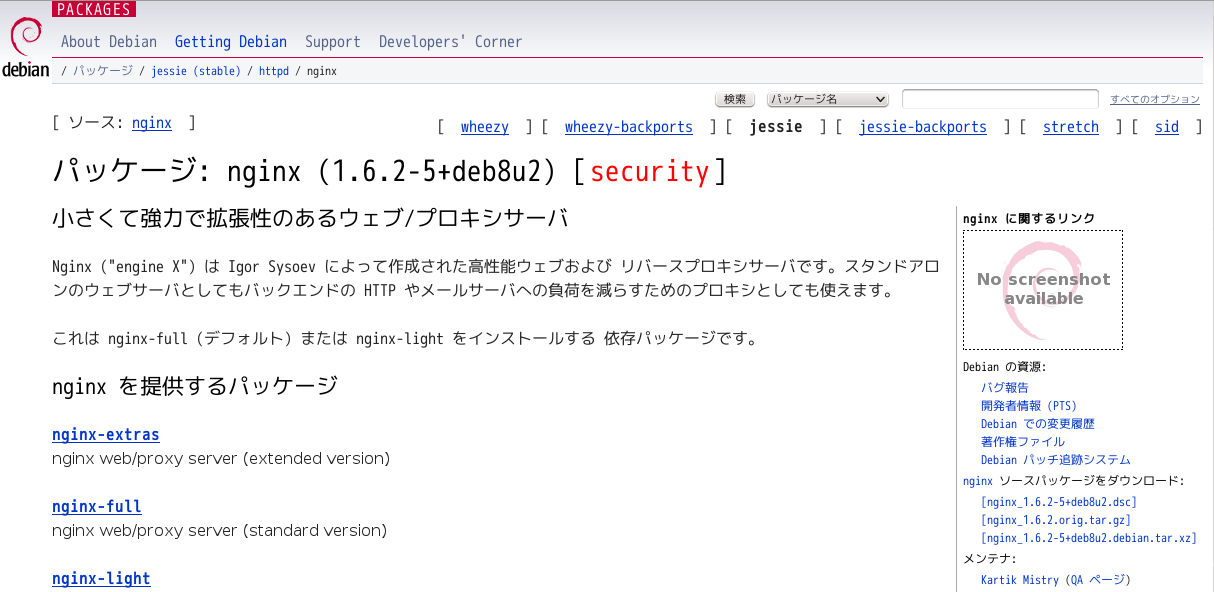
\includegraphics[width=0.9\hsize]{image201606/pdo.png}
   \end{center}
  \end{frame}
        

 \begin{frame}[containsverbatim]{control ファイルの中身}
  Package -- パッケージの名前 (例: \verb+Package: nginx+)
 \end{frame}

 \begin{frame}[containsverbatim]{control ファイルの中身}
  Maintainer -- パッケージのメンテナ

  例: \verb+Maintainer: Kartik Mistry <kartik@debian.org>+
 \end{frame}

 \begin{frame}[containsverbatim]{control ファイルの中身}
  Section -- パッケージの分類 (例: \verb+Section: httpd+)

  {\scriptsize{
admin         (管理ユーティリティ),					    
cli-mono      (Mono/CLI),						    
comm	      (コミュニケーションプログラム),				    
database      (データベース),						    
debug	      (デバッグパッケージ),					    
devel	      (開発),							    
doc	      (ドキュメント),						    
editors	      (エディタ),						    
education     (教育),							    
electronics   (電子工学),						    
embedded      (組み込みソフトウェア),					    
fonts	      (フォント),						    
games	      (ゲーム),						    
gnome	      (GNOME),						    
gnu-r	      (GNU R),						    
gnustep	      (GNUstep),						    
graphics      (グラフィック),						    
hamradio      (アマチュア無線),					    
haskell	      (Haskell),						    
httpd	      (ウェブサーバ),						    
interpreters  (インタプリタ),						    
introspection (Introspection),					    
java	      (Java),							    
kde	      (KDE),							    
kernel	      (カーネル),						    
libdevel      (ライブラリ開発),					    
libs	      (ライブラリ),						    
lisp	      (Lisp),							    
localization  (言語パック),						    
mail	      (メール),						    
math	      (数学),							    
metapackages  (メタパッケージ),					    
misc	      (その他),						    
net	      (ネットワーク),						    
news	      (ニュースグループ),					    
ocaml	      (OCaml),						    
oldlibs	      (旧式ライブラリ),					    
otherosfs     (異なるオペレーティングシステムやファイルシステムのもの),   
perl	      (Perl),							    
php	      (PHP),							    
python	      (Python),						    
ruby	      (Ruby),							    
science	      (科学),							    
shells	      (シェル),						    
sound	      (サウンド),						    
tasks	      (タスク),						    
tex	      (\TeX),							    
text	      (テキスト処理),						    
utils	      (ユーティリティ),					    
vcs	      (バージョン管理システム),				    
video	      (映像),							    
web	      (ウェブソフトウェア),					    
x11	      (X ウィンドウシステムのソフトウェア),			    
xfce	      (Xfce),							    
zope	      (Zope/Plone フレームワーク),				    
}}
 \end{frame}

 \begin{frame}[containsverbatim]{control ファイルの中身}
  Description -- パッケージの説明文

  \begin{itemize}
   
   \item Debian Policy 3.4
	 \begin{itemize}
	  \item 初めて見た人がインストールしたいか判断できるように書くべ
		しとされている
	  \item 重要なことは説明文の出だしに書くことになっている
	 \end{itemize}
   % \item control ファイルのDescriptionは英語
%	 英語の読めない人・苦手な人に翻訳が必要
%   \end{itemize}
  
% \begin{itemize}
 \item 1行目 -- short description (短い説明文)\\
       例:\\
       {
  \scriptsize
\begin{verbatim}
Description: small, powerful, scalable web/proxy server
\end{verbatim}
}
 \item 2行目以降 -- long description (長い説明文)\\
       例:\\
  \scriptsize
\begin{verbatim}
 Nginx ("engine X") is a high-performance web and reverse proxy server
 created by Igor Sysoev. It can be used both as a standalone web server
 and as a proxy to reduce the load on back-end HTTP or mail servers.
 .
 This is a dependency package to install either nginx-full (by default) or
 nginx-light.
\end{verbatim}
  \end{itemize}
 \end{frame}

  \begin{frame}{Description -- パッケージの説明文}
   control ファイルのDescriptionは英語

   Debian はコミュニティベースなので、誰かボランティアが翻訳する

   \pause
   \begin{itemize}
    \item パッケージになっているソフトウェアを知らないと正しく翻訳できない
    \item Universal なのでソフトウェアの分野(業界)が幅広く、少人数でやるのは困難
   \end{itemize}\pause
   ⇒ 自分の普段使っているパッケージ・自分の専門分野のパッケージなら翻訳できるはず!
  \end{frame}
 
\section{DDTP / DDTSS}
 \begin{frame}{DDTP -- Debian Description Translation Project}

 \url{http://ddtp.debian.net/}

  \begin{itemize}
   \item パッケージのDescriptionを翻訳するプロジェクト
   \item Debian 公式開発者でなくても作業できます
   \item 日本語チームの方針: 翻訳の品質を向上させること。量ではない
     {\scriptsize (でも原文の伸びはすごい…)}
  \end{itemize}

  \begin{center} 
  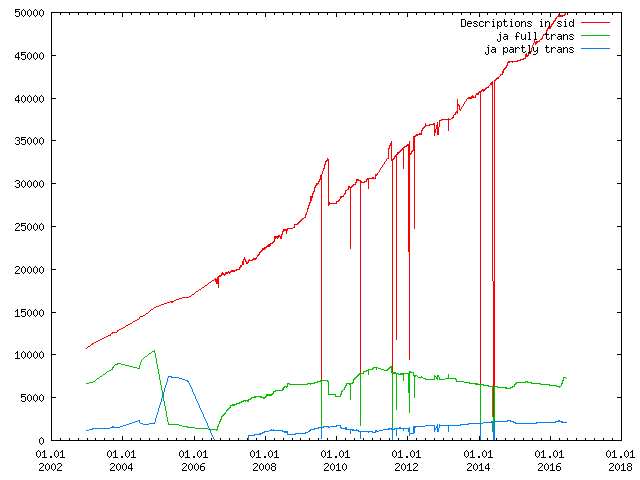
\includegraphics[width=0.65\hsize]{image201606/stat-trans-sid-ja.png}
  \end{center}

 \end{frame}

 \begin{frame}{DDTP -- Debian Description Translation Project}
   言語別統計

   \begin{center} 
  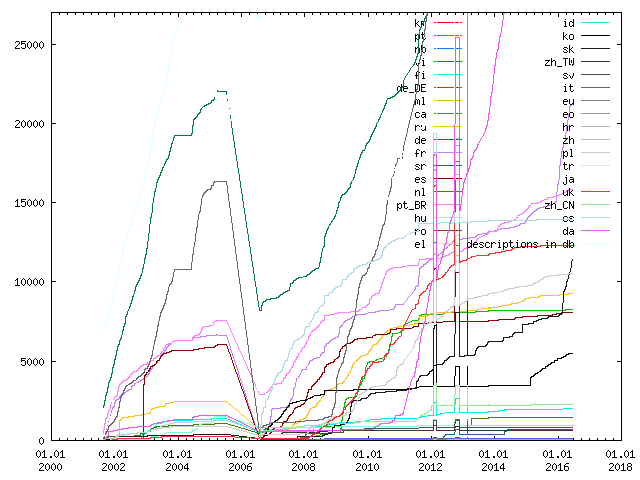
\includegraphics[width=0.9\hsize]{image201606/ddts-stat.png}
   \end{center}
 \end{frame}

 \begin{frame}{DDTP -- Debian Description Translation Project}
   言語別・Priority別統計

   \begin{center} 
  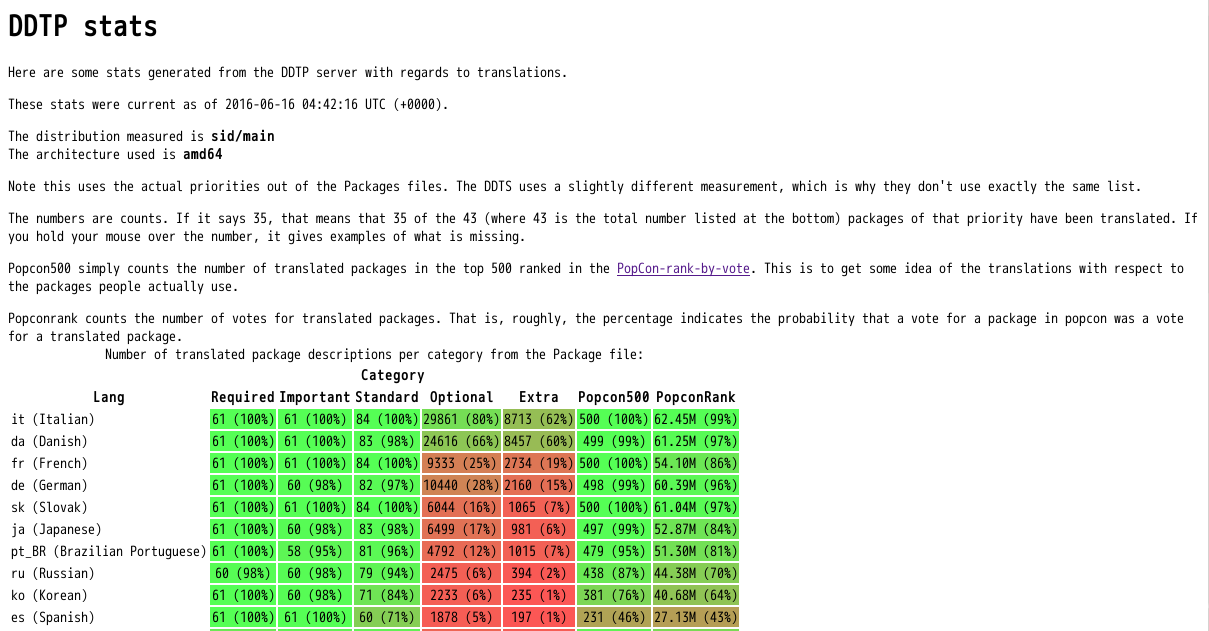
\includegraphics[width=\hsize]{image201606/stats-sid.png}
   \end{center}
 \end{frame}

 \begin{frame}{DDTSS}
   Web でDescriptionの翻訳・レビュー・修正ができるサイト\\
   日本語への翻訳は
   \url{http://ddtp.debian.net/ddtss/index.cgi/ja}

   \begin{center} 
  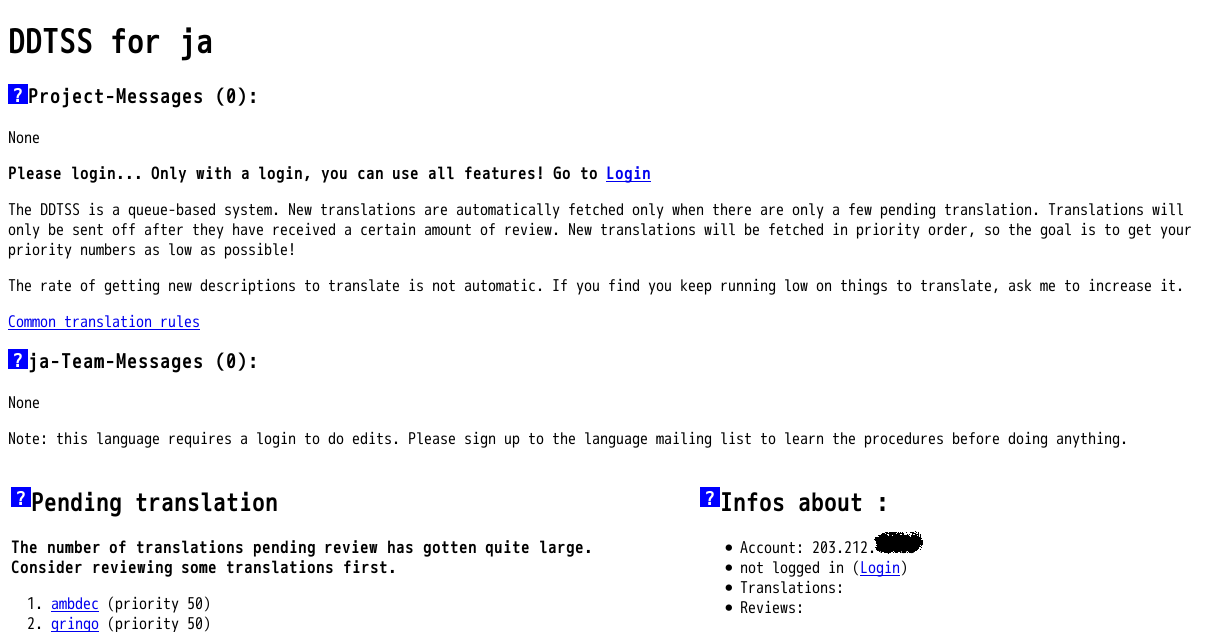
\includegraphics[width=0.9\hsize]{image201606/ddtss-anonymous.png}
   \end{center}
 \end{frame}

  \begin{frame}{DDTSS}
    Debian 公式開発者でなくても作業できます\\
    誰でもアカウントを作成して翻訳・レビュー・修正ができます

   詳しくは 第53回東京エリアDebian勉強会(2009年6月勉強会)の資料など\\
   \url{https://tokyodebian.alioth.debian.org/2009-06.html}

   \begin{center} 
  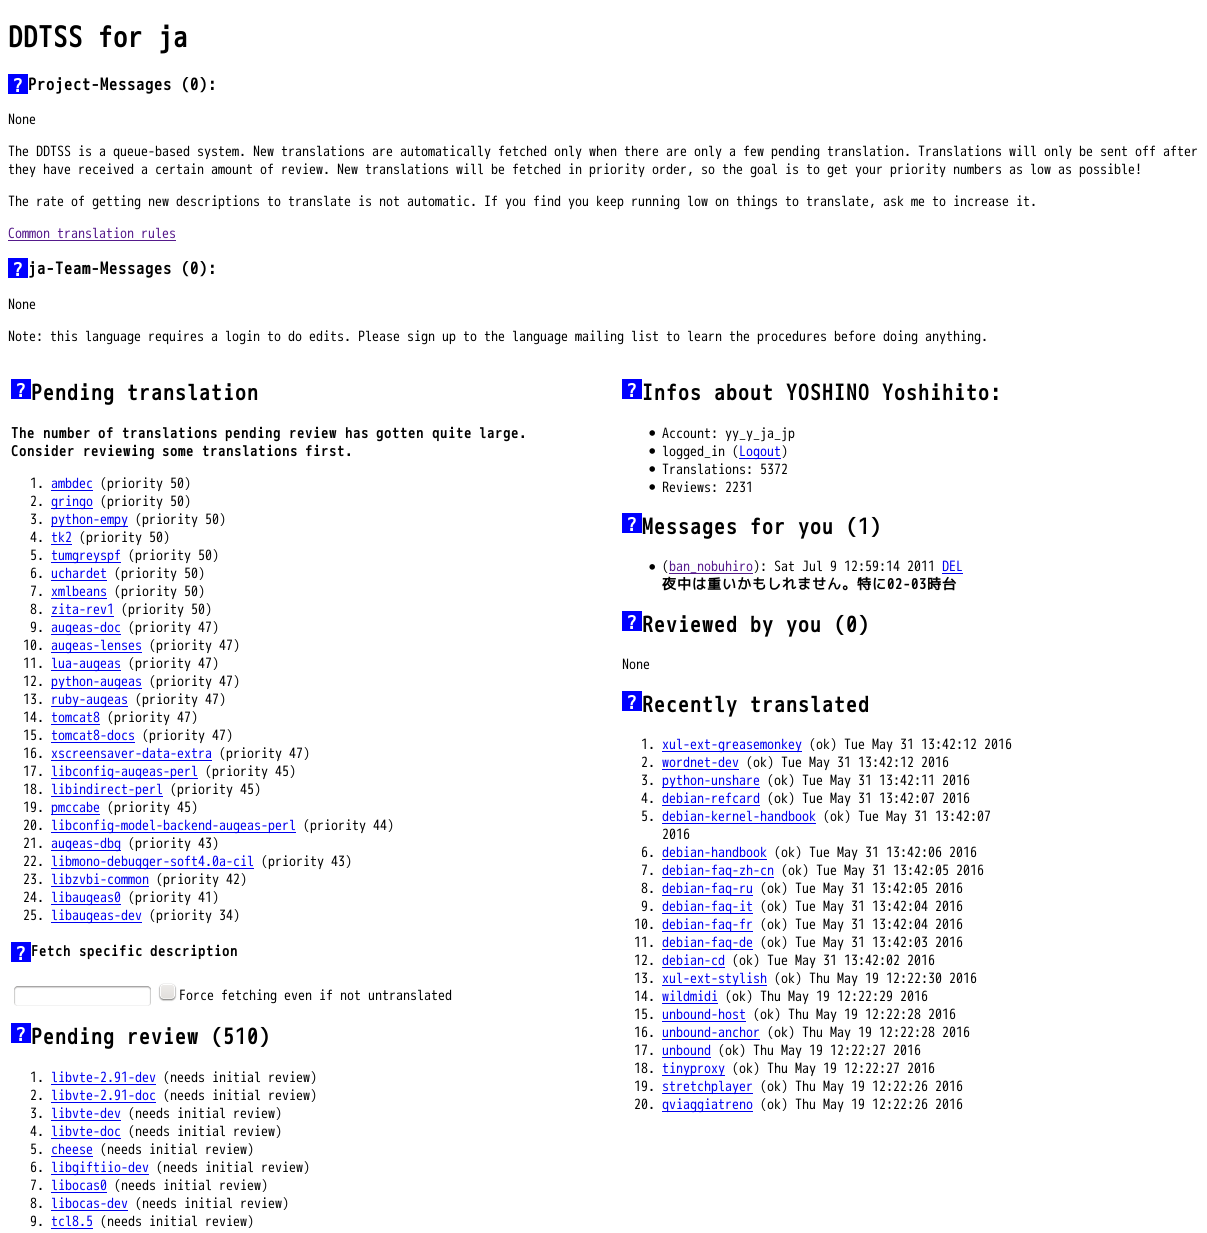
\includegraphics[width=0.9\hsize]{image201606/ddtss.png}
   \end{center}
 \end{frame}

 \begin{frame}{DDTSS}
  3人がレビューすると翻訳済みになり、その説明文が Debianのレポジトリに反映されます

  \begin{center} 
  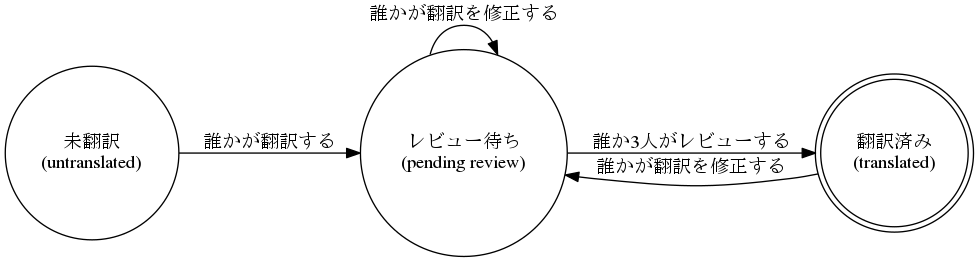
\includegraphics[width=0.9\hsize]{image201606/ddtss-flow.png}
   \end{center}
 \end{frame}

\section{まとめ}

\begin{frame}{まとめ}
 \begin{itemize}
  \item Debian は Universal な OS なので
	\begin{itemize}
	 \item 幅広い分野のソフトウェアのパッケージが多数ある\\
	   -- その中からインストールしたいものを選ぶきっかけとして、パッケージ名、説明文などがある
	 \item 様々な母国語・言語のユーザーが使う ⇒ 翻訳を提供
	\end{itemize}
      \item Debian はコミュニティベースなので基本ボランティア\\
        -- パッケージのメンテナンス、翻訳、…
  \item 日本語チームとしては、質の高い日本語でパッケージ説明文を日本語ユー
	ザーに提供したい
  \item DDTSS で誰でも説明文の翻訳ができます
  \item パッケージのソフトウェアやその分野(業界)を知らないと翻訳ができない。質の高い翻訳もできない\\\pause
    ⇒ ユーザーのみなさん、お使いのパッケージの翻訳・レビュー・修正にご協力ください!\\
    みなさん、あなたの専門分野のパッケージの翻訳・レビュー・修正にご協力ください!
 \end{itemize}
\end{frame}

\frame{\titlepage{}}

\section{補足1}

\begin{frame}{}
\end{frame}

 \begin{frame}{質問}
  DDTSS にアクセスしてみたいのですが、つながりません。\\
  \pause
  ⇒ はい、5月からつながりません。今のところ /etc/hosts に次の行を追加してください。

  117.121.245.169 ddtp.debian.net
 \end{frame}

 \begin{frame}[containsverbatim]{質問}
  \scriptsize
  \url{https://lists.debian.org/debian-i18n/2016/05/msg00008.html}
  \begin{verbatim}
To: Ivan Masar <helix84@centrum.sk>
Cc: Debian Internationalization <debian-i18n@lists.debian.org>
Subject: Re: DDTSS down
From: Martijn van Oosterhout <kleptog@gmail.com>
Date: Mon, 23 May 2016 22:42:08 +0200
Message-id: <CADWG95uYBfu-73rqy9wR3XUwe3tyyuD8vLE1UQmR17-TUnorcA@mail.gmail.com>
In-reply-to: <CAGdvKqgJsV2bDQ5dqB0oAJNoS9xCw71WKgAtvM38MvSU=sc4zg@mail.gmail.com>
References: <CAGdvKqg3b-axEjbSmif5nsJRkiUDRFSSUY0CGJtPv2hMO1KJVA@mail.gmail.com> <CADWG95tvaSYZB=cv9SjZjOMQm6k93x9dKn5HXF071u+t60ysrQ@mail.gmail.com> <CAGdvKqgJsV2bDQ5dqB0oAJNoS9xCw71WKgAtvM38MvSU=sc4zg@mail.gmail.com>

I've been in communication with Andreas and Thomas the last few days. 
The IP address changed because the host moved. So some stuff needed to 
be updated.

The machine is up again at the new IP address 117.121.245.169. The DNS 
however still needs to be updated. Not sure what is required to fix 
that, but what we tried so far hasn't worked yet.

Nearly there though..

Have a nice day,
\end{verbatim}
 \end{frame}

\section{補足2}

 \begin{frame}{質問}
    \pause
  \begin{itemize}
  \item 小学生でも英語が必修なのに、翻訳する意味はあるのですか?\\
    \pause
    ⇒ パッケージのメンテナは英語が苦手な人にも使ってもらいたいと思っているでしょう。
    \pause
   \item 私の専門分野のパッケージはありますが、日本語はオワコンです。翻
	 訳する意味はあるのですか?\\
    \pause
	 ⇒ 英語が苦手な人でもパッケージを使ってくれるようになれば、その人があな
	 たの専門分野に興味を持ってくれる可能性が高まると思います。
    \pause
   \item 私の専門分野にある最近の用語には日本語訳がありません。\\
    \pause
	 ⇒ その用語の部分はカタカナが業界的に通用しているならカタカナで、そうでないなら無理に訳さず英語のままでいいと思います。
  \end{itemize}
 \end{frame}

\end{document}

;;; Local Variables: ***
;;; outline-regexp: "\\([ 	]*\\\\\\(documentstyle\\|documentclass\\|emtext\\|section\\|begin{frame}\\)\\*?[ 	]*[[{]\\|[]+\\)" ***
;;; End: ***
